\documentclass[10pt,conference]{IEEEtran}
\IEEEoverridecommandlockouts

\usepackage{cite}
\usepackage{amsmath,amssymb}
\usepackage{graphicx}
\usepackage{booktabs}
\usepackage{url}
\usepackage{tikz}
\usetikzlibrary{positioning,arrows.meta}

\begin{document}

\title{Semantic Mutation Testing for Auditing\\ AI Data-Engineering Benchmarks}

\author{\IEEEauthorblockN{Anonymous Author(s)}
\IEEEauthorblockA{Anonymous Institution\\
Email: anonymous@example.org}}

\maketitle

\begin{abstract}
Execution-based benchmarks drive progress measurement for AI agents that generate
data transformations. Their evaluators face two opposing error directions:
\emph{representation false rejection}, where an acceptable output is rejected
because it is represented differently, and \emph{semantic false acceptance}, where
an output encoding a different meaning is accepted. Recent evaluator validation has
primarily targeted the first. We introduce \emph{semantic mutation testing}, a
meta-evaluation method that provides a controlled way to probe the second. A perturbation changes exactly
one declared semantic property and is admitted only when it provably changes the
output; a matched conventional edit then modifies \textbf{the same cells of the
same table} with an arbitrary value, so that detection can be compared without
confounding which cells were chosen. Auditing two divergent evaluator
implementations of ELT-Bench over 180 released output tables, we find structured
semantic-risk probes are substantially less detectable than matched arbitrary
edits: excluding one parsing-level case, one implementation rejects 34 of 34
arbitrary edits and 0 of 34 structured semantic edits to the same cells (exact
$p\!=\!1.2\times10^{-10}$), while the other rejects all 68. Controlled ablation
attributes survivors to named mechanisms, including two redundant row-set
mechanisms that erase output population and grain before any cell is compared, so
a single comparator patch would not restore sensitivity. The protocol, operator
catalogue, advance predictions and analysis plan were cryptographically frozen
before execution, and the artifact runs without a cloud warehouse.
\end{abstract}

\begin{IEEEkeywords}
benchmark validity, mutation testing, evaluator meta-evaluation, data
engineering, construct validity
\end{IEEEkeywords}

\section{Introduction}

Benchmarks for AI data-engineering agents execute a generated transformation and
compare its output against stored ground truth \cite{eltbench,spider2,bird}. The
comparison function is the operative definition of correctness, so its properties
matter as much as the tasks.

Recent work shows these functions are often \emph{too strict}. Audits of
text-to-SQL benchmarks report pervasive errors that penalise correct outputs
\cite{annotationerrors}, and an audit of ELT-Bench attributed a third of
column-level mismatches to the benchmark, motivating a corrected release with
normalisation for booleans, numeric tolerance, percentage formats, null
representation and row ordering \cite{eltverified}. This is
\textbf{representation false rejection}: acceptable output, evaluator rejects.

The opposite direction is barely measured. \textbf{Semantic false acceptance} is
semantically different output that the evaluator accepts. The two are coupled:
every normalisation that removes a false rejection enlarges the equivalence class
the evaluator treats as one answer, and nothing guarantees the enlargement stops
at representation.

\begin{quote}
\emph{An evaluator can become more robust to harmless representational variation
while simultaneously becoming less discriminative with respect to structured
semantic differences.}
\end{quote}

Existing validation compares evaluator verdicts against human equivalence
judgements on \emph{observed} agent outputs \cite{eltverified}. That design
detects false rejections, since rejected-but-equivalent pairs occur naturally. It
cannot efficiently detect false acceptances, which must be constructed. Prior work
documents \emph{which} normalisations reduce false rejection; our contribution is
a method that quantifies the \emph{discrimination cost} of those normalisations
using admissibility-backed perturbations and matched controls.

Mutation testing supplies the instrument. Mutants are seeded faults used to assess
whether a test suite detects them \cite{jiaharman,mutationsurvey}, adapted to SQL
with operators over clauses, operators, NULL handling and identifiers \cite{tuya}.
We raise it a level: the artifact assessed is the benchmark evaluator, and the
seeded faults change declared \emph{semantic} properties rather than syntax.

\textbf{Contributions.} (i) Semantic mutation testing as a meta-evaluation method,
with admissibility rules and same-cell matched controls; (ii) a frozen,
literature-grounded catalogue of 22 operators over six families, each registering
an advance prediction; (iii) an audit of two pinned ELT-Bench evaluator
implementations, with mechanism-level attribution by controlled ablation; (iv) an
artifact, frozen by hash before execution, that runs without a cloud warehouse.

The corrections we audit were introduced for documented reasons and validated
against human judgement \cite{eltverified}. We do not claim they are mistakes.

\section{Method}
\label{sec:method}

\subsection{Definitions}

Let $P$ be a transformation and $I$ a database state. A \textbf{semantic mutant}
$P'$ changes exactly one declared semantic property of $P$ while remaining
plausible, and is \textbf{admissible} only with a witness state $I_w$ where
$P(I_w)\neq P'(I_w)$, compared exactly and never with the evaluator under test.
The experimental unit is (subject, operator, witness, evaluator version), since a
normalisation may fire only on data of a particular shape.

We distinguish two levels. At \emph{transformation level} (Arm A) an actual SQL
edit plus witness establishes the distinction, and we use the term semantic
mutant. At \emph{output level} (Arm B) we perturb released output tables; we call
these \textbf{evaluator probes} or \textbf{structured semantic-risk
perturbations}, and we do not claim each corresponds to a demonstrated naturally
occurring SQL fault.

\subsection{Operators and freezing}

Operators are organised by the property violated, not the construct edited:
grain/cardinality \cite{kimball}, measures, population, temporal, absence
\cite{codd}, representative-value. Each declares preconditions, mutation rule,
witness requirements, affected columns, expected distinction, and an advance
prediction. The catalogue, predictions, witness rules and analysis plan were
hashed before the confirmatory run; 16 of 22 operators are predicted
\emph{rejected}, so the catalogue is not filtered by expected outcome. We did not
register externally, so we describe this as pre-specified and cryptographically
frozen, not as preregistration.

\subsection{Same-cell matched controls}

A detection rate alone cannot distinguish a selectively semantics-blind evaluator
from a uniformly permissive one. Each probe is paired with a conventional edit
\cite{tuya} perturbing \emph{the same cells of the same table} in the same
magnitude bin, using an arbitrary constant or scale factor carrying no
data-modelling meaning. This within-instance pairing licenses the selectivity
claim: the evaluator sees an identically-shaped edit in both cases.

For version $v$, $\mathrm{SMDR}_v$ and $\mathrm{CMDR}_v$ are the fractions of
admissible semantic and control instances rejected, and $\Delta_v$ their
difference.

\section{Experimental Design}

\subsection{Subject and evaluator versions}

ELT-Bench \cite{eltbench} scores its transformation stage by column-wise
comparison against stored outputs over 203 data models. Two divergent evaluator
implementations exist in the public repository; we pin both by commit SHA and file
hash, treat evaluator version as a first-class factor, and call them
\emph{default} and \emph{Verified}. Neither is described as canonical.
Table~\ref{tab:evals} summarises their comparison semantics, recovered from the
pinned sources. Both are driven through their real load path, writing outputs to
CSV and reading them back, because parser coercion is itself part of evaluator
behaviour.

\begin{table}[t]
\caption{Comparison semantics of the two pinned implementations.}
\label{tab:evals}
\centering\footnotesize
\begin{tabular}{@{}lll@{}}
\toprule
& \textbf{default} & \textbf{Verified} \\
\midrule
Row handling & sort by declared key & drop duplicates, then \\
             &                      & intersect on inferred key \\
Numeric      & rel.\ tol.\ $10^{-2}$ & rel.\ tol.\ $10^{-2}$ \\
Null vs.\ zero & distinct & equivalent \\
Normalisation & none & quotes, timestamps, \\
              &      & booleans, percentage scale \\
\bottomrule
\end{tabular}
\end{table}

\subsection{Two arms}

Transformation SQL is not published for the full benchmark: the repository's
evaluation queries are extraction statements and ground truth ships as output
CSVs. We use two arms and never pool their claims.

\textbf{Arm B (primary, output level).} Probes are applied to 180 released
benchmark output tables spanning 90 models, pinned by commit. Six of the 22
frozen operators admit a faithful output-level realisation, yielding seven probes
because absence is probed in both directions; the remaining 16 are recorded
\textsc{not\_realizable}, because their semantics live in the computation and
imitating them by editing an output would degenerate into arbitrary corruption,
which the protocol forbids.

\textbf{Arm A (fidelity anchor, transformation level).} The same frozen operators
are applied as SQL edits to three repository-provided transformations whose output
schemas match their task specifications exactly (\texttt{shipping.drivers},
\texttt{retails.cus\-tomers}, \texttt{retails.nations}), on witnesses built from the
frozen structural requirements. We have \emph{not} verified that these reproduce
the benchmark ground-truth CSVs, which are not retrievable in our environment, so
we do not call them validated references. Arm A establishes that Arm B's
distinctions are realisable by plausible SQL edits; it is not a prevalence
estimate.

\section{Results}
\label{sec:results}

\subsection{RQ1: discriminative power}

Over 468 admissible probe instances per version, $\mathrm{SMDR}$ is 80.1\%
$[76.3,83.5]$ for default and 2.8\% $[1.6,4.7]$ for Verified. Applicability varies
sharply---row-multiplicity probes apply to 175 of 180 tables, tie probes to
4---so per-operator denominators, not the pooled rate, carry the claim
(Table~\ref{tab:main}).

\begin{table}[t]
\caption{Arm B. Probe detection by operator and version; $n$ is admissible
instances per version.}
\label{tab:main}
\centering\footnotesize
\begin{tabular}{@{}llrrr@{}}
\toprule
\textbf{Probe} & \textbf{Family} & \textbf{$n$} & \textbf{default} & \textbf{Verified} \\
\midrule
GC1  & grain          & 175 & 100.0\% & 0.6\% \\
PP1  & population     & 162 & 100.0\% & 6.8\% \\
RV1  & repr.\ value   & 4   & 100.0\% & 25.0\% \\
ME3  & measures       & 10  & 100.0\% & 0.0\% \\
AB1  & absence        & 12  & 100.0\% & 0.0\% \\
AB1R & absence        & 12  & 100.0\% & 0.0\% \\
AB2$^\dagger$ & absence & 93 & 0.0\% & 0.0\% \\
\midrule
\textbf{Pooled} & & 468 & 80.1\% & 2.8\% \\
\bottomrule
\end{tabular}
\\[2pt]
\footnotesize$^\dagger$parsing-level case, analysed separately in \S\ref{sec:parse}.
\end{table}

\subsection{RQ2: selectivity at comparator level}

Excluding AB2, whose distinction is erased before comparison, the comparator-level
result is unambiguous: \textbf{the Verified implementation rejects 34 of 34
arbitrary matched edits and 0 of 34 structured semantic edits to the same cells}
(34 discordant pairs, all one direction; exact two-sided
$p=1.2\times10^{-10}$). The default implementation rejects 34 of 34 in
\emph{both} conditions. That the same edits are fully detected by one
implementation and never by the other shows that the observed separation is
evaluator-specific rather than an artifact of which cells were perturbed. The
semantic standing of the edits rests instead on the declared operator semantics,
their literature grounding, the admissibility rule, and their transformation-level
realisation in Arm~A.

Including AB2, value-level figures are 0/127 versus 125/127. Among \textbf{row-set}
probes, $\Delta_{\text{Verified}}=+2.6$ points with 9 discordant pairs, below our
pre-specified threshold for testing; there the evaluator is not selectively but
\emph{uniformly} blind, erasing row-set differences whether or not they carry
meaning.

\textbf{Exploratory robustness.} A post-hoc check, not part of the frozen design,
replaces each control with an \emph{in-distribution} value observed elsewhere in
the same column (or a permutation of that column), preserving dtype and empirical
support. Across 32 eligible pairs the separation is unchanged: Verified rejects
32 of 32 in-distribution controls and 0 of 32 semantic edits
($p=4.7\times10^{-10}$); default rejects both at 32 of 32. Control detectability
therefore cannot be attributed to out-of-distribution values.

\subsection{Parsing-level erasure}
\label{sec:parse}

AB2 replaces null with the sentinel \texttt{'N/A'} and is rejected by
\emph{neither} implementation (0/93 each), because \texttt{read\_csv} coerces the
sentinel back to null during the evaluator's own load. A reviewer may reasonably
regard \texttt{'N/A'} as another representation of missingness; we therefore
report it separately and exclude it from the comparator claim. It remains
instructive: permissiveness is a property of the whole evaluation pipeline, not
only of its comparator, and this was our one incorrect advance prediction.

\subsection{RQ3: mechanisms}

Survivors are attributed by disabling one mechanism at a time through a
single-anchor patch on the pinned comparator, requiring survival when enabled and
rejection when that mechanism alone is disabled. Of 359 survivors, 150 are
attributed to key-based intersection, 24 to null/zero equivalence, 12 to duplicate
removal and 10 to percentage-scale normalisation.

Row multiplicity resists single-mechanism attribution: 163 of 174 survivors are
rejected by neither ablation alone, because duplicate removal and key intersection
are each independently sufficient. Joint ablation rejects 39 of 39 in a random
40-table sample---a mechanism study, not a population estimate. The practical
consequence is that \emph{a single comparator patch would not restore row-set
sensitivity}.

The most consequential mechanism is structural, not numeric: alignment intersects
and deduplicates both row sets before any cell is compared
(Fig.~\ref{fig:align}), so differences in output population and grain are removed
from the comparison rather than measured by it.

\begin{figure}[t]
\centering
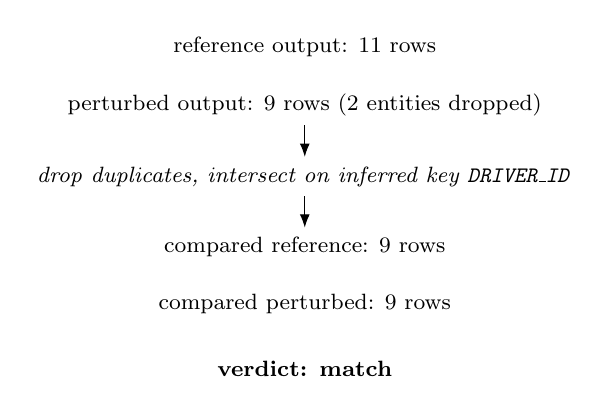
\begin{tikzpicture}[font=\footnotesize,node distance=2.2mm]
\node (gt) {reference output: 11 rows};
\node (mu) [below=of gt] {perturbed output: 9 rows (2 entities dropped)};
\node (ar) [below=4mm of mu] {\textit{drop duplicates, intersect on inferred key \texttt{DRIVER\_ID}}};
\node (cg) [below=4mm of ar] {compared reference: 9 rows};
\node (cm) [below=of cg] {compared perturbed: 9 rows};
\node (v) [below=3.5mm of cm] {\textbf{verdict: match}};
\draw[-{Latex}] (mu) -- (ar);
\draw[-{Latex}] (ar) -- (cg);
\end{tikzpicture}
\caption{Measured instance (\texttt{shipping.drivers}, Verified). A probe removing
18\% of the output population is accepted: row-set differences are erased before
cell comparison.}
\label{fig:align}
\end{figure}

\subsection{Arm A and leakage control}

Across the three transformations, 22 operator sites were applicable, 44
operator/subject pairs were recorded \textsc{not\_applicable}, 4 were inadmissible
on their witness, leaving 18 admissible semantic mutants with matched controls.
Verified rejects 6 of 18 against 15 of 18 controls ($\Delta=+50.0$); default
rejects 16 of 18 against 18 of 18. The families that survive in Arm B survive
here, confirming the distinctions are realisable by transformation-level edits.
Verdicts vary with the witness---percentage-scale normalisation fires only with
sufficient rows, so ME3 survives on one subject and is rejected on another---which
is why survival is reported per tuple rather than per operator.

An earlier exploratory pilot was written with knowledge of evaluator source; its
rates are excluded from every claim above and reported only in the artifact. Six
of seven confirmatory probes share a semantic property with that pilot, so we
stratify: the one probe with no pilot history yields 0/93 under Verified against
13/375 for the rest. Advance predictions, frozen before execution, hold for 77.4\%
of instances, the exception being AB2. Decisively, the selectivity result of
\S\ref{sec:results}-B is a within-instance contrast on the same cells of the same table: operator
foreknowledge may explain which cells were selected, but cannot explain why the
evaluator accepts one edit and rejects the matched edit when both touch the same
cells.

\section{Discussion}

\subsection{Trade-off, not verdict}

These results measure evaluator permissiveness, not benchmark quality.
Normalisations that reduce representation false rejection are valuable and were
validated against human judgement \cite{eltverified}; what was missing is a
measurement of their cost in semantic false acceptance. Semantic mutation testing
supplies it cheaply enough to run as a regression check whenever a comparison rule
changes, and we recommend evaluator patches report both directions. The mechanisms
we probe---key-based alignment, null normalisation, numeric tolerance and CSV
round-tripping---are not specific to the audited benchmark, so the catalogue is
designed to transfer to other execution-based evaluators.

\subsection{Threats}

\textbf{Corpus provenance.} Arm B uses released benchmark output tables rather than
the distributed ground-truth CSVs, unreachable in our environment. Provenance
affects realism of schema and value distribution, not the validity of comparing a
table with its perturbation; re-running on ground truth is a path change.
\textbf{Arm B fidelity.} Output perturbations need not correspond to naturally
occurring query faults; claims are scoped to evaluator sensitivity, and Arm A
anchors realisability.
\textbf{Subject provenance.} Arm A subjects match their task specifications but
were not verified against ground-truth outputs; we avoid calling them validated
references.
\textbf{Coverage.} Only six of 22 operators are realisable at output level,
yielding seven probes, and temporal operators appear only in Arm A.
\textbf{Uneven applicability.} Per-operator denominators are reported precisely
because the pooled rate mixes operators applying to 4 and to 175 tables.
\textbf{Witness dependence.} Survival is a property of the full tuple; Arm B
supplies witness diversity through 180 distinct tables.
\textbf{Operator selection.} The catalogue is literature-derived, frozen and hashed
before running, includes operators predicted rejected, and one prediction failed.
\textbf{Control comparability.} Conventional operators overlap the absence family
by construction \cite{tuya}; absence probes use non-null controls, and the
exploratory in-distribution check addresses the out-of-distribution objection.
\textbf{Arm A size.} Eighteen instances over three subjects is an anchor, not an
estimate.

\subsection{Artifact}

The artifact contains the freeze manifest with commit SHAs and file hashes,
snapshots of both comparison layers, the frozen catalogue and predictions, witness
rules, per-instance records for both arms, ablation patches and analysis scripts.
Extraction of the comparison layer is checked byte-identical against the pinned
sources, so verdicts cannot come from a reimplementation. Everything runs locally
without a cloud warehouse.

\section{Conclusion}

Evaluator tolerance has at least two error directions, and validating only one
leaves the other unmeasured. Semantic mutation testing provides a controlled way to
probe the second, by seeding changes to declared semantic properties, admitting
them only when they provably change the output, and contrasting them with
arbitrary edits to the same cells. On two pinned ELT-Bench evaluators it finds a near-total comparator-level
dissociation under one implementation and none under the other, and attributes
survivors to specific alignment, normalisation and parsing mechanisms---one of
them redundant, so no single patch restores sensitivity. Benchmark evaluators
should be validated on both directions.

\begin{thebibliography}{99}
\footnotesize
\bibitem{eltbench} T.~Jin, Y.~Zhu, and D.~Kang, ``ELT-Bench: An end-to-end benchmark for evaluating AI agents on ELT pipelines,'' \emph{Proc. VLDB Endow.}, vol.~19, no.~2, pp.~84--98, 2025.
\bibitem{eltverified} C.~Zanoli, A.~Giovannini, T.~Jin, A.~Klimovic, and Y.~Perlitz, ``ELT-Bench-Verified: Benchmark quality issues underestimate AI agent capabilities,'' arXiv:2603.29399, 2026.
\bibitem{annotationerrors} T.~Jin, Y.~Choi, Y.~Zhu, and D.~Kang, ``Pervasive annotation errors break text-to-SQL benchmarks and leaderboards,'' \emph{Proc. VLDB Endow.}, vol.~19, no.~5, pp.~931--944, 2026.
\bibitem{tuya} J.~Tuya, M.~J.~Su\'arez-Cabal, and C.~de~la~Riva, ``Mutating database queries,'' \emph{Inf. Softw. Technol.}, vol.~49, no.~4, pp.~398--417, 2007.
\bibitem{jiaharman} Y.~Jia and M.~Harman, ``An analysis and survey of the development of mutation testing,'' \emph{IEEE Trans. Softw. Eng.}, vol.~37, no.~5, pp.~649--678, 2011.
\bibitem{mutationsurvey} M.~Papadakis, M.~Kintis, J.~Zhang, Y.~Jia, Y.~Le~Traon, and M.~Harman, ``Mutation testing advances: An analysis and survey,'' \emph{Adv. Comput.}, vol.~112, pp.~275--378, 2019.
\bibitem{kimball} R.~Kimball and M.~Ross, \emph{The Data Warehouse Toolkit}, 3rd~ed. Wiley, 2013.
\bibitem{codd} E.~F.~Codd, ``Extending the database relational model to capture more meaning,'' \emph{ACM Trans. Database Syst.}, vol.~4, no.~4, pp.~397--434, 1979.
\bibitem{spider2} F.~Lei \emph{et al.}, ``Spider 2.0: Evaluating language models on real-world enterprise text-to-SQL workflows,'' in \emph{Proc. Int. Conf. Learning Representations (ICLR)}, 2025.
\bibitem{bird} J.~Li \emph{et al.}, ``Can LLM already serve as a database interface? A big bench for large-scale database grounded text-to-SQLs,'' in \emph{NeurIPS}, 2023.
\end{thebibliography}

\end{document}
